\section{实验设计与结果分析}
\label{sec8:exp}

在这一节中,我们评估了本章提出的算法在不同参数设置和多种数据集下的表现情况。所有算法均使用C++17实现,并用g++编译器以-O3优化级别进行编译。所有的代码均运行在Intel Xeon Gold 6258R @ 2.70GHz的CPU上,内存为128GB。在所有算法中,默认使用三角核函数作为默认核函数,并采用Dijkstra算法计算最短路径距离。

\subsection{数据集介绍}

我们使用了四个具有不同规模和类别的数据集,相关参数列在表~\ref{tab:datasets}中,$\vert V \vert$和$\vert E \vert$ 分别表示路网图的点数和边数,$\vert N \vert$表示数据点数量,$N / \vert E \vert$ 平均每条边上的数据点数量。所有路网数据均从OSMnx包从OpenStreetMap上下载获得。每条边都被假设为一条直线,并且每个数据点会被匹配到距离最近的边上。数据点的来源包括包括报警记录、付费停车记录和出租车行程记录。

\begin{table}[h]
\centering
\def\arraystretch{1.5}
\caption{数据集参数}
\label{tab:datasets}
\begin{tabular}{c|c|c|c|c} 
\hline
数据集     & $\vert V \vert$ & $\vert E \vert$ & $N$ & $N / \vert E \vert$  \\ 
\hline \hline
Berkeley    & 1576            & 4378            & 735366          & 168                              \\ 
\hline
Johns Creek & 3074            & 3471            & 979072          & 282                              \\ 
\hline
San Francisco  & 9700         & 16008           & 5379023         & 336                              \\ 
\hline
New York	& 55765           & 92229           & 38400730        & 416                              \\ 
\hline
\end{tabular}
\end{table}

\subsection{RFS算法和已有工作的对比}

首先,我们评估了我们提出的带有线段点共享优化的区间森林法(RFS)在生成精确核密度值时的效率,并与基线算法——最短路径共享算法(SPS)和最优算法——聚合距离增强算法(ADA)进行对比。SPS算法只采用最基本的最短路径共享框架,而不会建立任何索引;ADA算法会每次根据时间窗口过滤所有的数据点,并建立线性索引。

每组测试包含多轮不同的时间窗口查询,并且以在线的形式给出,即必须实时对于每个查询立刻返回结果。每个时间窗口默认包含 $70\%$ 的数据点。

\begin{figure*}[p!]\centering
	\hspace{-8pt}
	\scalebox{0.3}[0.3]{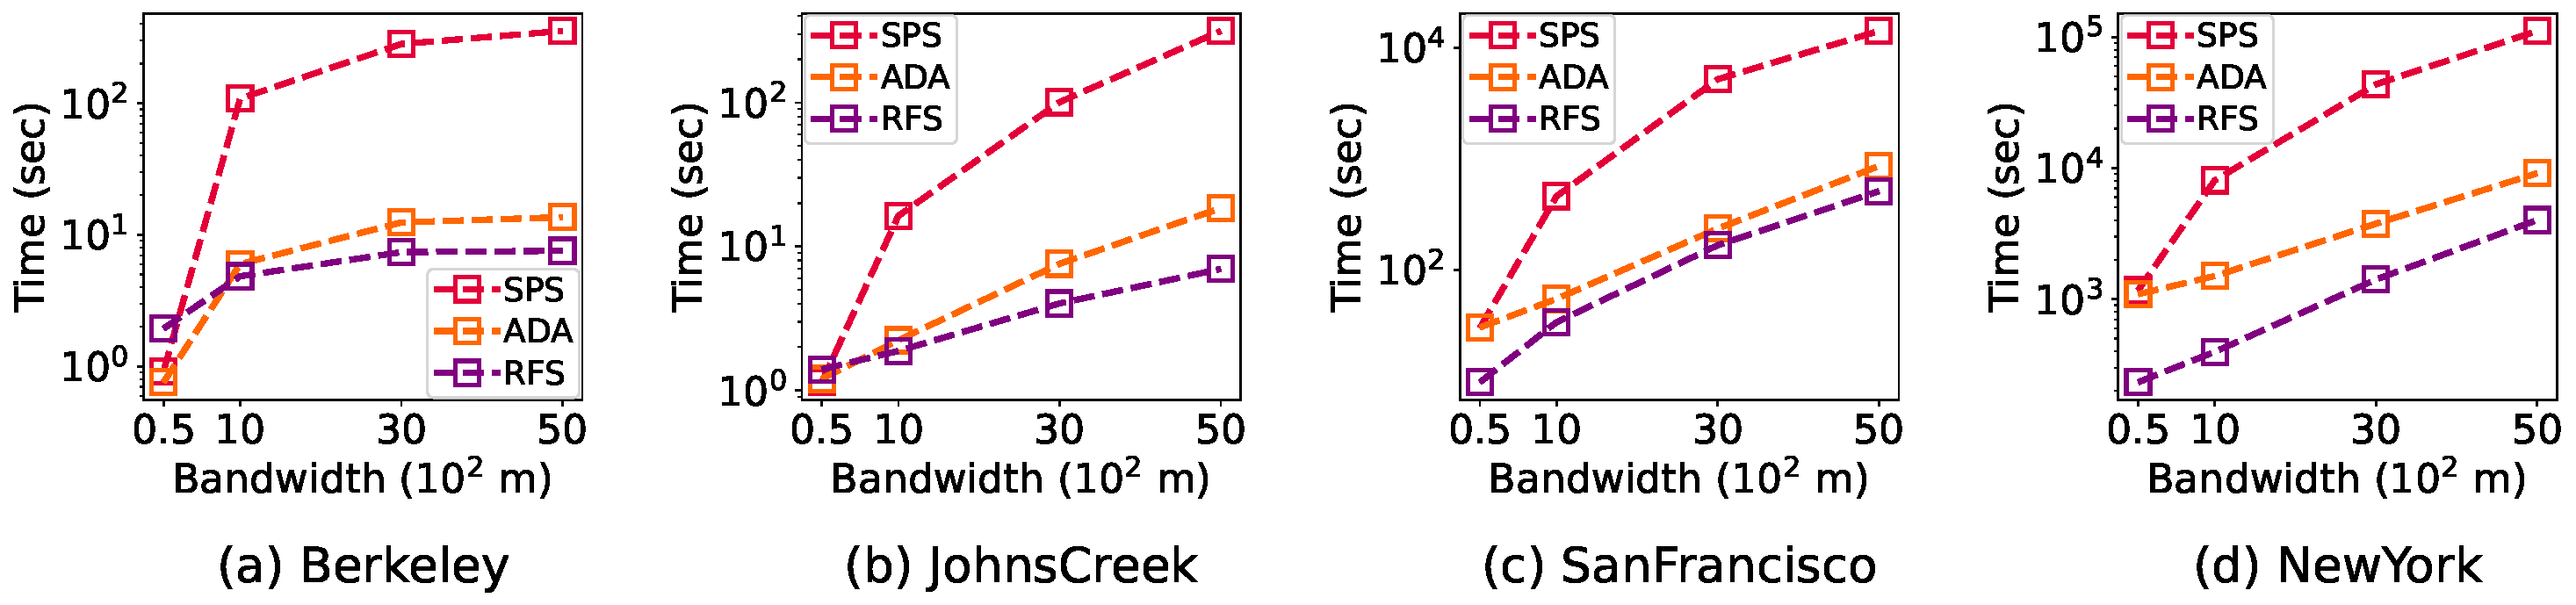
\includegraphics{./figures/EXP_Bandwidth_R.pdf}}
	\vspace{-8pt}
	\caption{不同空间范围带宽(50m,1000m,3000m,5000m)下的处理时间。}
	\label{exp1.1}
	
	\vspace{10pt}
	\scalebox{0.3}[0.3]{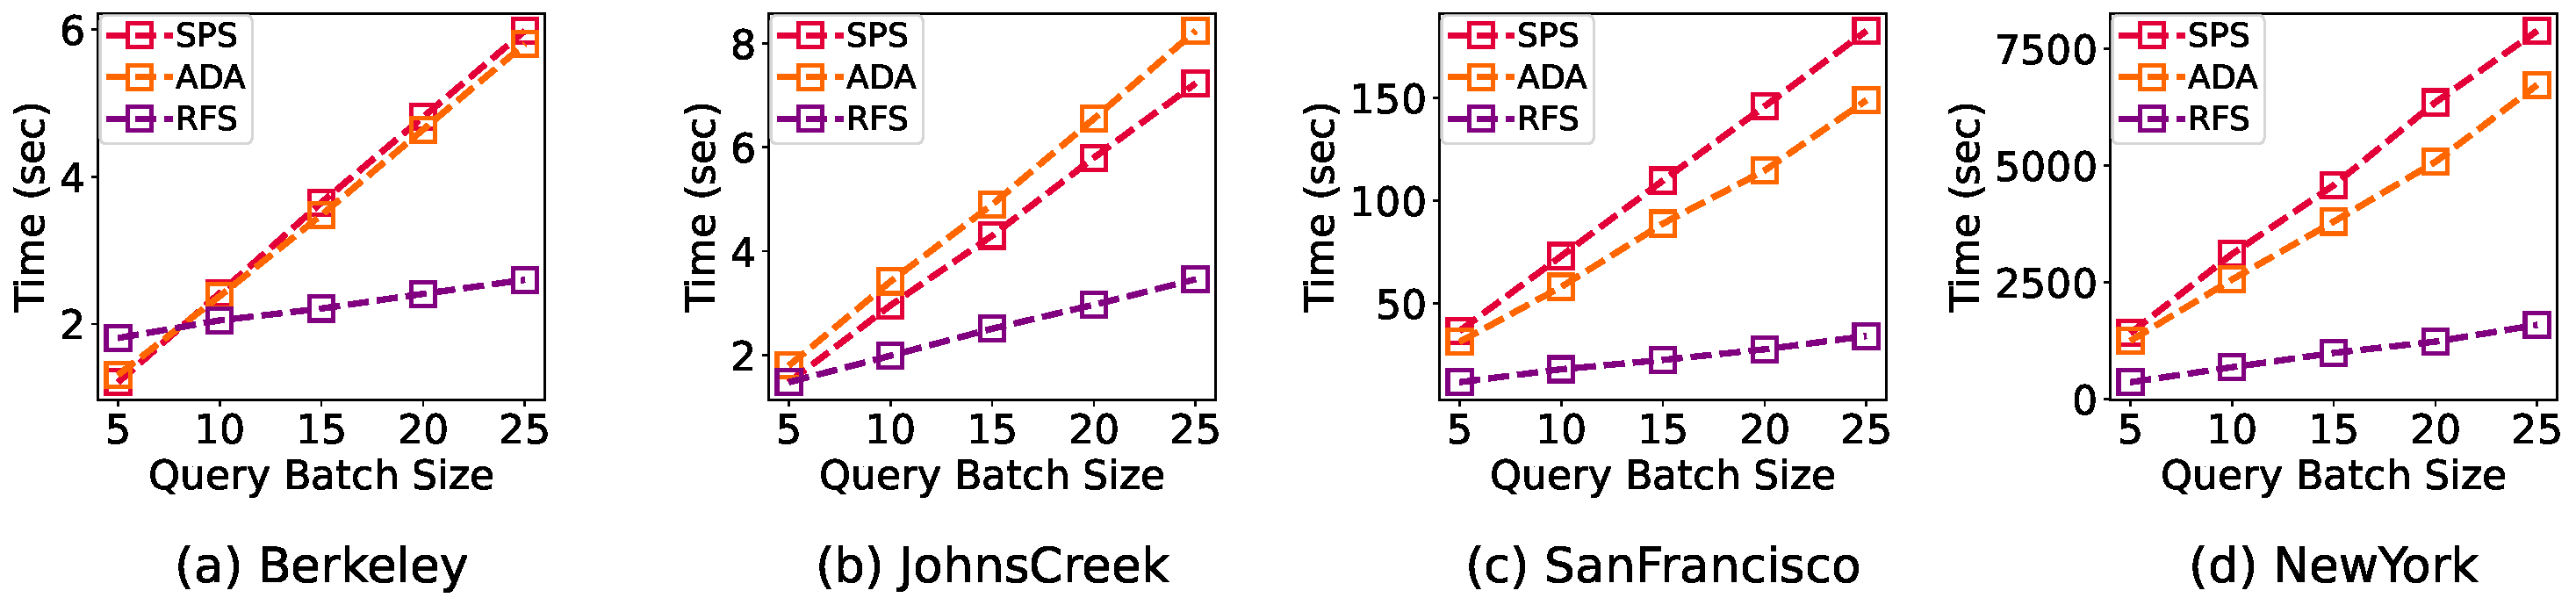
\includegraphics{./figures/EXP_Bandwidth_W.pdf}}
	\vspace{-8pt}
	\caption{不同查询数量(5,10,15,20,25)下的处理时间。}
	\label{exp1.2}
	
	\vspace{10pt}
	\scalebox{0.3}[0.3]{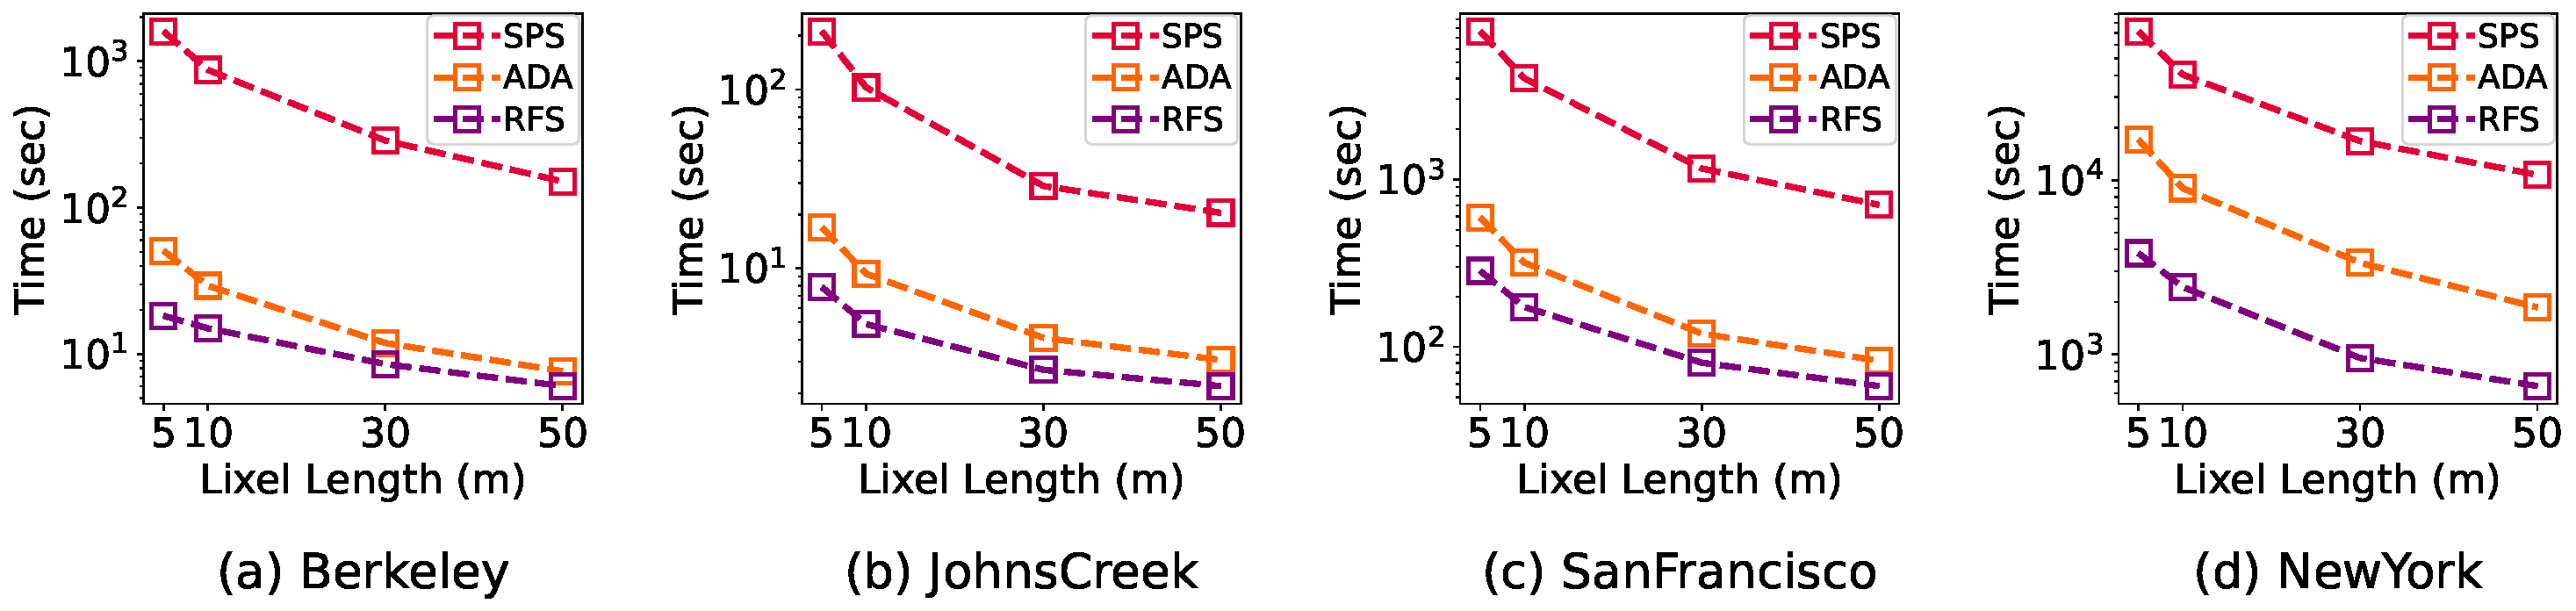
\includegraphics{./figures/EXP_Bandwidth_L.pdf}}
	\vspace{-8pt}
	\caption{不同线段点长度(5m,10m,30m,50m)下的处理时间。}
	\label{exp1.3}
	
	\vspace{10pt}
	\scalebox{0.3}[0.3]{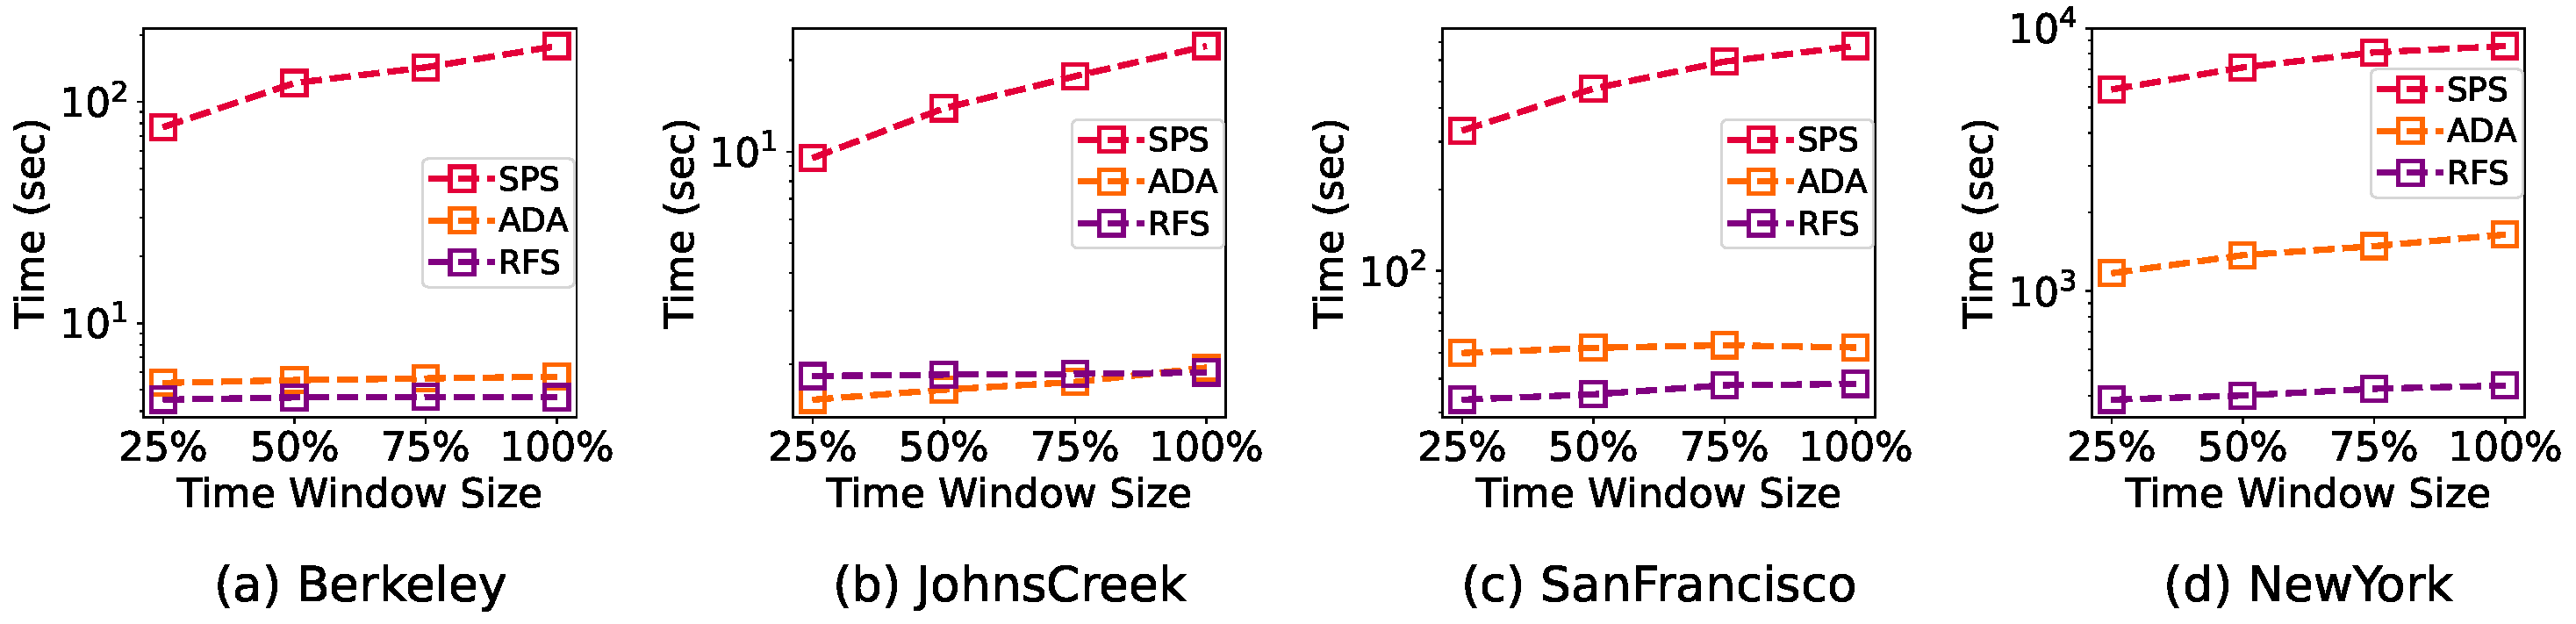
\includegraphics{./figures/EXP_Bandwidth_P.pdf}}
	\vspace{-8pt}
	\caption{不同时间窗口大小(25\%,50\%,75\%,100\%)下的处理时间。}
	\label{exp1.4}
\end{figure*}


\textbf{以范围带宽为自变量。} 首先,我们在四个数据集中使用单组查询(而不是多组查询)评估不同带宽(50米、1000米、3000米、5000米)下的处理时间。线段点的长度设置为10米,这是一个合适的分辨率。

结果以对数形式展示在图~\ref{exp1.1} 中。没有索引的SPS算法比其他基于索引的方法慢1到2个数量级,尤其是在较大带宽的情况下。RFS算法相比ADA算法最多可实现6倍的加速,但在较小网络和较低带宽的情况下表现不佳,这是因为在索引构建上花费了过多的时间。

\textbf{以多轮查询次数为自变量。} 前面的实验是对单个查询设计的。然而对于多轮查询,ADA算法必须针对不同的时间窗口重建索引。因此,我们测试了不同查询次数对结果的影响,查询轮数分别为5、10、15、20、25。空间带宽设置为50米,线段点长度为50米。在这种情况下,重新加载和索引所有事件将耗费较多的时间。

图~\ref{exp1.2} 显示了所有方法的时间都呈现出线性增长的趋势,其中截距代表索引构建时间,而斜率则代表每次查询的处理时间。RFS算法在小数据集(例如 Berkeley)上的预处理时间相对于查询的时间较高,但其增长比率远低于 SPS 和 ADA,导致总的处理时间依然较少。对于其他三个数据集,RFS算法在所有情况下表现得更好。

\textbf{以线段点长度为自变量。} 线段点的长度直接决定了分辨率。对于一个粗略的快速视图,50米的线段点已经足够,因为平均边长只有100米到200米。然而,用户可能为了提高分辨率而设置更小的线段点长度。在这部分实验中,线段点长度分别为5米、10米、30米和50米。每个查询批次包含5个时间窗口。

图 \ref{exp1.3} 以对数形式展示了不同的线段点长度(5米、10米、30米、50米)下的处理时间。所有结果显示了大致的反比关系,因为较小的线段点长度会导致更多的线段点被创建,从而增加计算开销。与其它方法相比,RFS算法表现出显著的优势,特别是在较低的线段点长度下,相比于ADA算法的速度提升高达4.5倍。 

\textbf{以时间窗口大小为自变量。} 我们还希望了解数据点规模如何影响查询效率,因此我们设置了不同大小的时间窗口,分别为总事件数的25\%、50\%、75\%和100\%。

如图~\ref{exp1.4} 所示,SPS算法的处理时间与数据点数量呈线性关系,因此随着时间窗口大小的增加,处理时间也随之增加。相反,RFS算法的处理效率与时间窗口大小无关。ADA算法则略有不同,因为时间窗口大小仅影响预处理步骤,但不影响后续查询步骤。因此,即使事件数量增加,RFS算法的效率也不会受到影响。

\textbf{内存开销。} 图~\ref{exp1.5} 展示了三种算法的内存使用情况。由于SPS算法不需要任何额外的空间,其内存使用量可以视为数据集本身的大小。其他两种算法(RFS算法和ADA算法)的内存使用仅与数据点数量相关。RFS算法在构建森林索引时仅需消耗相当于ADA算法3倍和SPS算法8倍的内存。考虑到复杂的索引结构,这样的内存开销是可以接受的。

\begin{figure}[h]\centering
	\scalebox{0.6}[0.6]{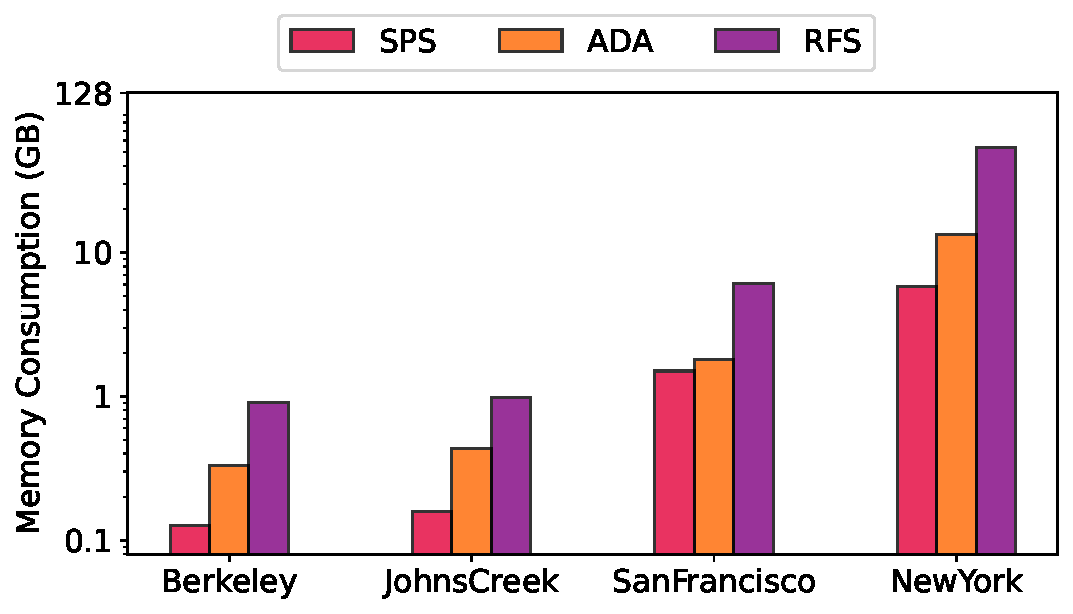
\includegraphics{./figures/EXP_Memory.pdf}}
	\caption{不同算法消耗的内存对比。}
	\label{exp1.5}
\end{figure}


\subsection{DRFS算法的高效性和有效性}

这一节评估了动态区间森林算法(DRFS)在不同的区间森林高度 $H$ 下的高效性和有效性。为了进行比较,我们使用了没有线段点共享优化的RFS算法,它具有静态结构。实验选择了两个带宽范围:1000米和20000米,线段点长度固定为50米,时间窗口包含了所有事件。算法初始设置 $H=1$,并逐步增加深度以展示其动态过程。

\textbf{高效性。} 为了说明索引和处理过程中的时间消耗,图~\ref{exp2.1} 和图~\ref{exp2.2} 分别展示了索引时间和处理时间。即使当 $H=10$ 时,DRFS算法构建索引所需的时间也很少,并且在大数据集(例如 NewYork)上甚至比RFS算法更快。大约来说,RFS算法的效果等同于$H \approx 8$的DRFS算法。在处理时间方面,不同的高度$H$之间没有显著差异。由于在一个查询批次中索引部分只执行一次,即使$H$较大,DRFS算法在高效性上依然表现良好。

\begin{figure}[h]\centering
	\scalebox{0.5}[0.5]{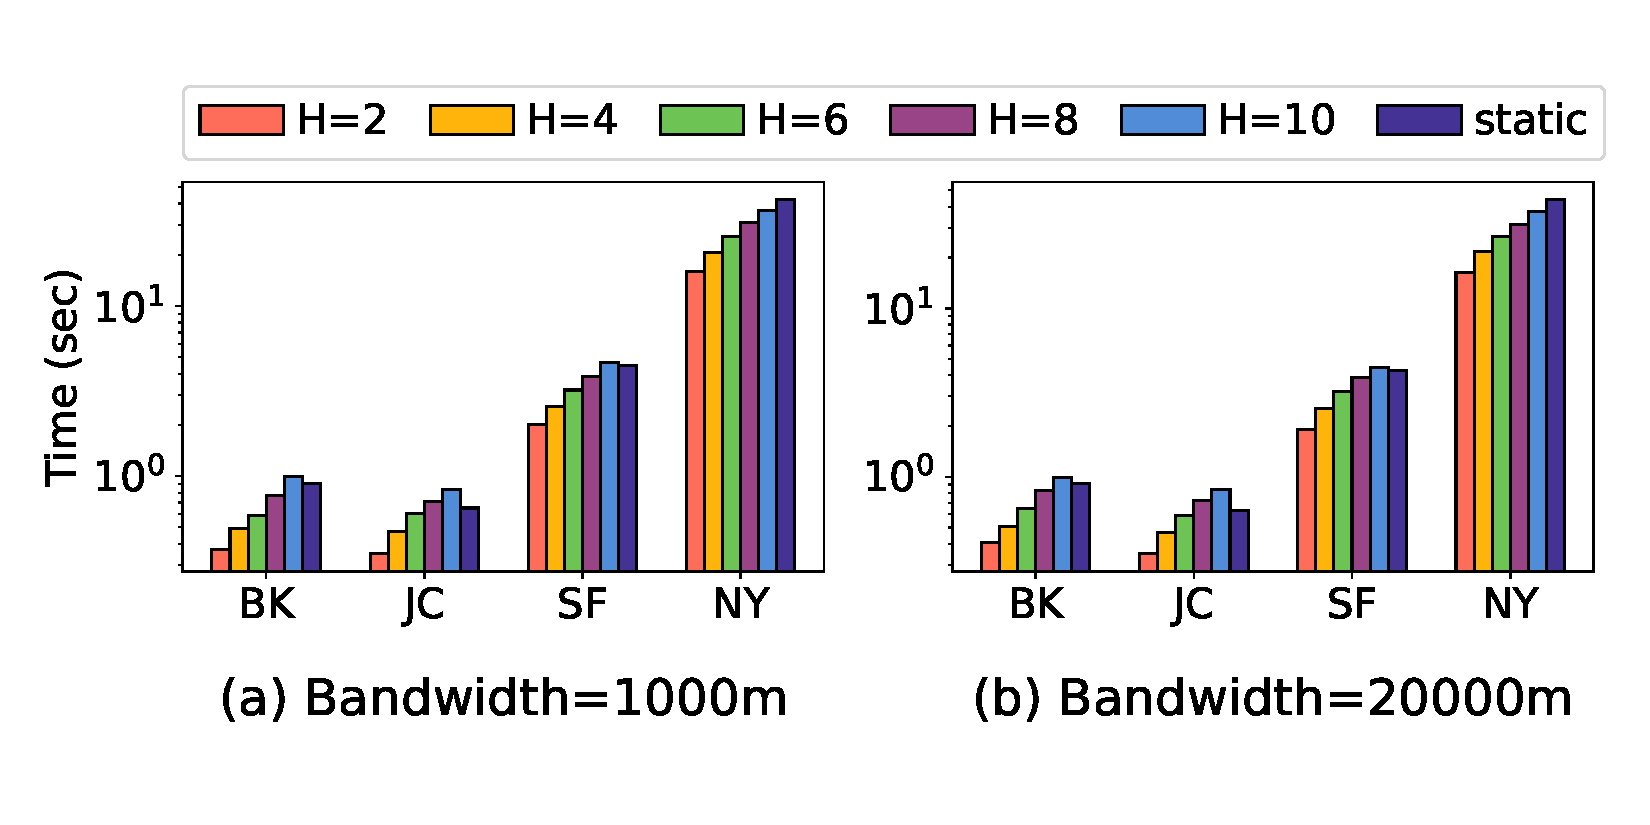
\includegraphics{./figures/EXP_H_PrepareTime.pdf}}
	\vspace{-1em}
	\caption{不同高度 $H$ 所需要的索引时间对比。}
	\label{exp2.1}
\end{figure}

\begin{figure}[h]\centering
	\vspace{-1em}
	\scalebox{0.5}[0.5]{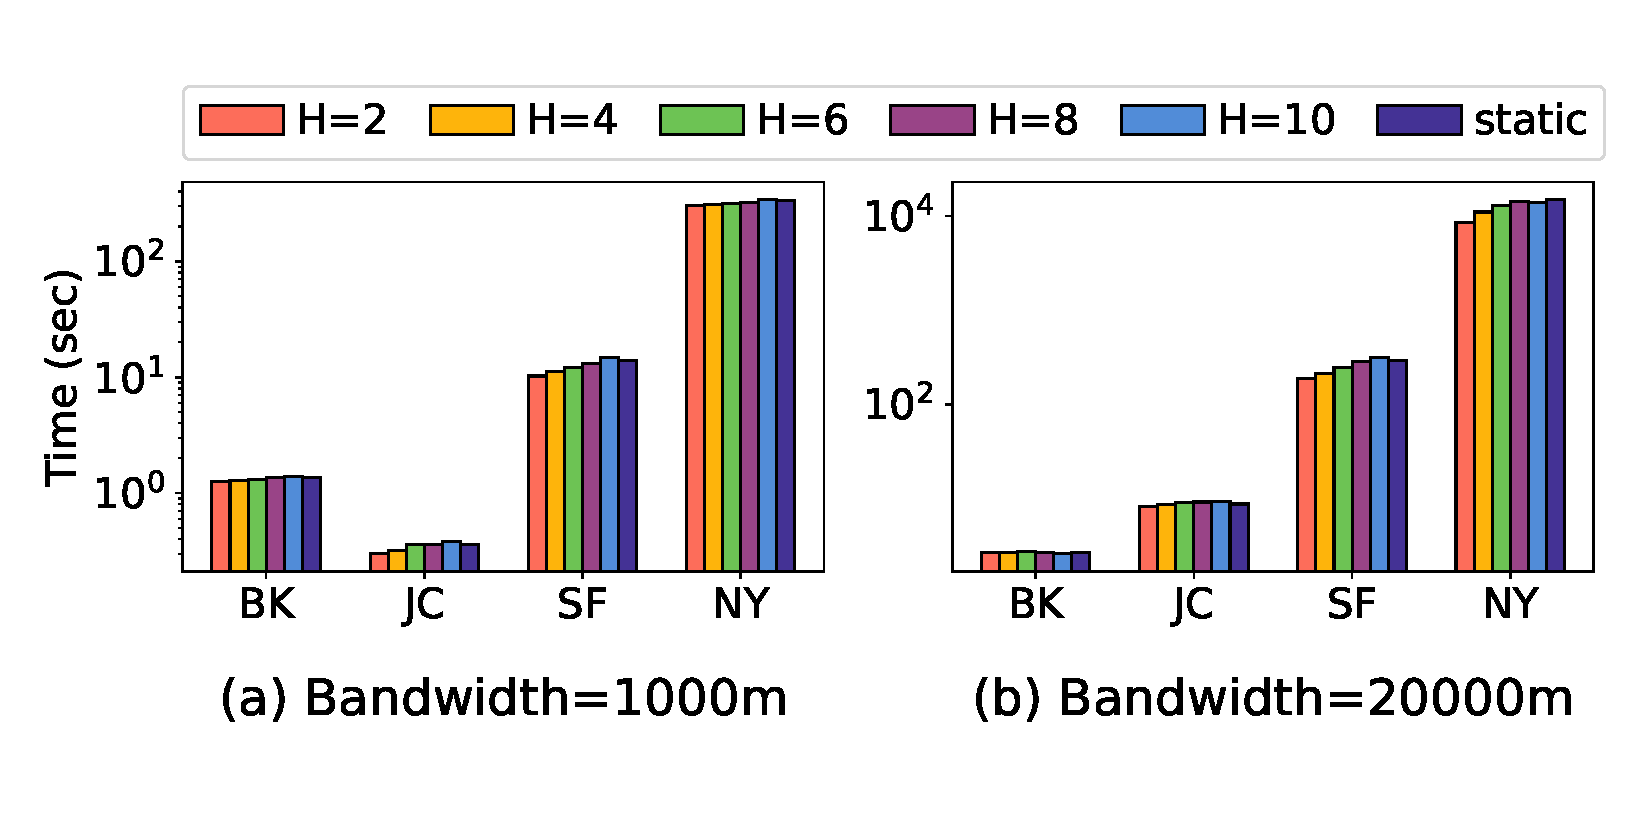
\includegraphics{./figures/EXP_H_RunningTime.pdf}}
	\vspace{-1em}
	\caption{不同高度 $H$ 下的查询时间对比。}
	\label{exp2.2}
\end{figure}

\textbf{有效性。} 由于DRFS算法是一种近似算法,我们也需要考虑其有效性,即计算出的核密度值是否准确。所有实验报告的准确率结果如图~\ref{exp2.3}所示。即使在 $H=2$ 的情况下,准确率仍然超过94\%。此外,随着 $H$ 的增加,准确性迅速提升,当 $H=10$ 时,所有四个数据集上的准确率均超过了99.9\%。

\begin{figure}[h]\centering
	\scalebox{0.5}[0.5]{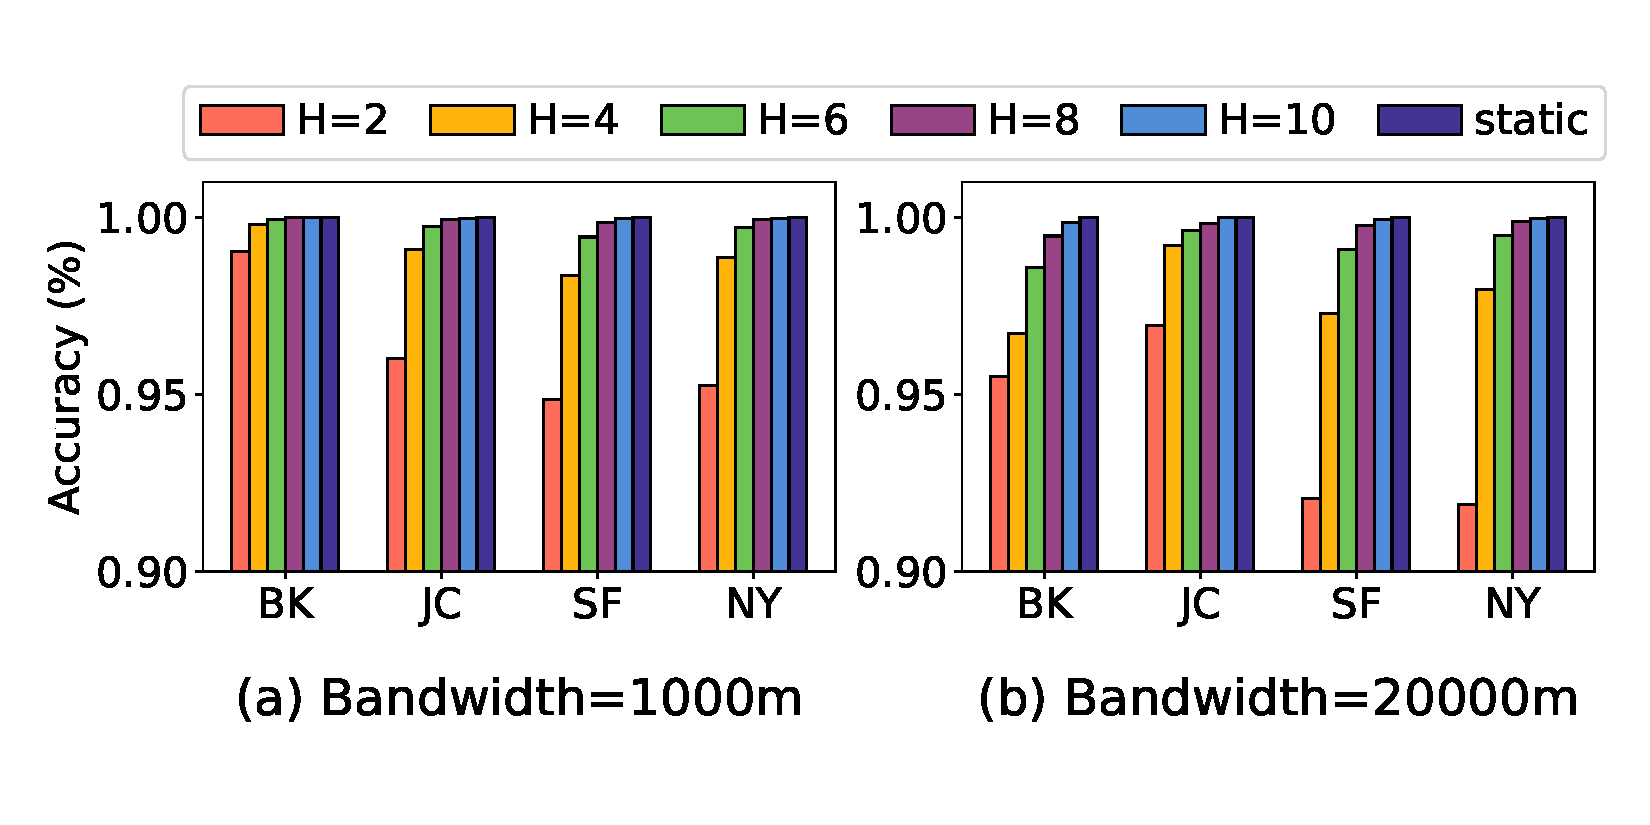
\includegraphics{./figures/EXP_H_Accuracy.pdf}}
	\vspace{-1em}
	\caption{不同高度 $H$ 下的答案准确度对比。}
	\label{exp2.3}
\end{figure}

\textbf{内存开销。}  图~\ref{exp2.4} 显示了两种算法的内存开销,这反映了索引的大小。其趋势与图~\ref{exp2.1} 类似,等效边界同样是 $H \approx 8$。当 $H=2$ 时,内存消耗接近ADA算法,表明我们量化策略的可行性。此外,内存使用的增长比率几乎是线性的且可以预测,这可以帮助用户选择合适的参数 $H$。

\begin{figure}[h]\centering
	\scalebox{0.5}[0.5]{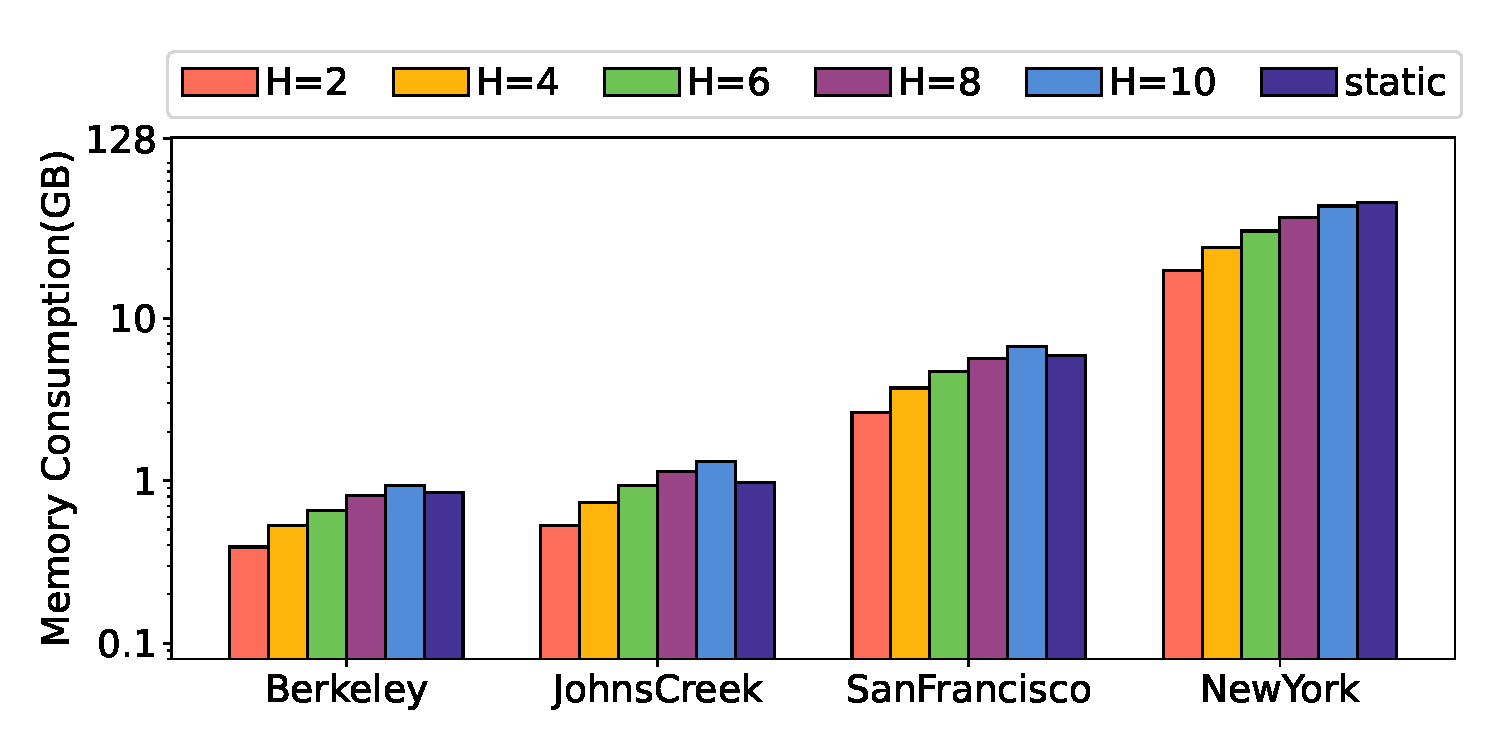
\includegraphics{./figures/EXP_H_Memory.pdf}}
	\caption{不同高度 $H$ 所需要的内存开销对比。}
	\label{exp2.4}
\end{figure}


综合考虑所有这些方面,实验表明DRFS算法具有很高的实用性。较小的 $H$ 值可以显著节省时间,并且仍然能够产生相对准确的结果;而较大的 $H$ 值仅需稍微多一点的时间即可生成几乎相同的结果。因此,用户可以根据需要选择合适的$H$值,并动态调整它。

\subsection{不同的核函数}
	
	该算法框架的另一个特点是可替换的核函数。由于使用不同核函数的所有计算过程都具有 $O(1)$ 的时间复杂度,因此它们可以在相同的时间内生成热力图。

	图~\ref{fig:exp_kernel} 展示了使用三角核函数、余弦核函数和指数核函数生成的三个不同的热力图。每个热力图上方都有其对应的函数图,所有密度值都被归一化处理。具体来说,余弦核函数的值始终大于指数核函数的值,而指数核函数的值又大于三角核函数的值,且斜率从高到低的依次是三角核函数、指数核函数和余弦核函数,这与结果的平滑度有关。此外,三角形核函数没有截断,而余弦和指数核函数在 $\pm 1$ 处被截断,这导致结果更加集中且边界更加明显。


\begin{figure}[h]\centering
	\begin{minipage}{0.3\linewidth}
	\centering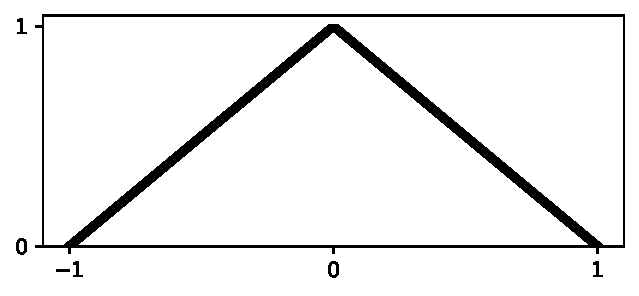
\includegraphics[height=20mm, width=45mm]{./figures/EXP_kernel_T.pdf}
	\end{minipage}
	\begin{minipage}{0.3\linewidth}
	\centering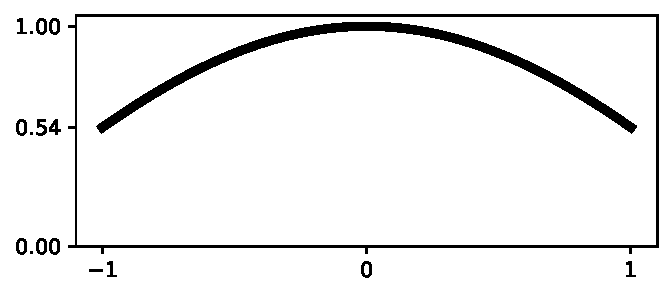
\includegraphics[height=20mm, width=45mm]{./figures/EXP_kernel_C.pdf}
	\end{minipage}
	\begin{minipage}{0.3\linewidth}
	\centering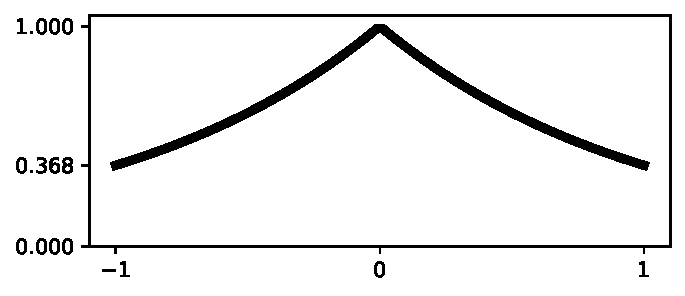
\includegraphics[height=20mm, width=45mm]{./figures/EXP_kernel_E.pdf}
	\end{minipage}
	
	\begin{minipage}{0.3\linewidth}
	\centering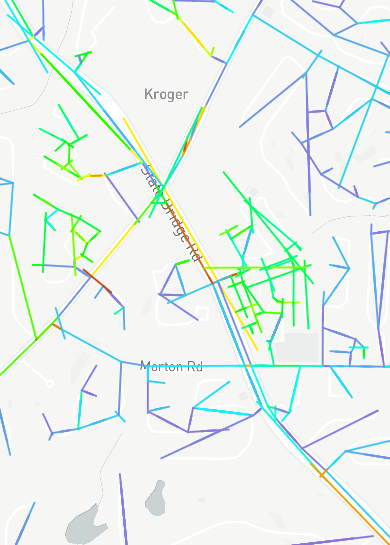
\includegraphics[height=48mm, width=36mm]{./figures/EXP_kernel_Triangular.PNG}
	\caption*{(a) 三角核函数}
	\end{minipage}
	\begin{minipage}{0.3\linewidth}
	\centering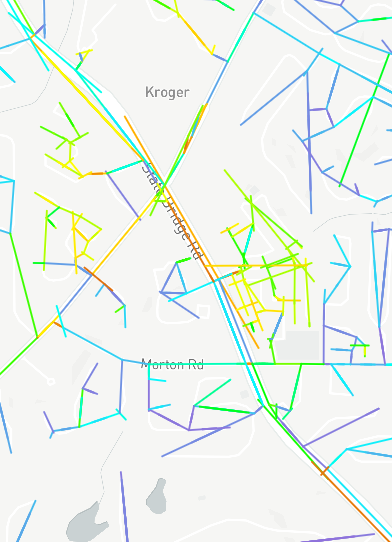
\includegraphics[height=48mm, width=36mm]{./figures/EXP_kernel_Cosine.PNG}
	\caption*{(b) 余弦核函数}
	\end{minipage}
	\begin{minipage}{0.3\linewidth}
	\centering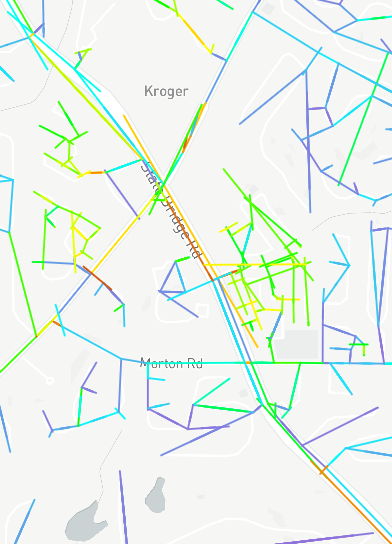
\includegraphics[height=48mm, width=36mm]{./figures/EXP_kernel_Exponential.PNG}
	\caption*{(c) 指数核函数}
	\end{minipage}
	\vspace{8pt}
	\caption{应用不同核函数的热力图结果。}
	\label{fig:exp_kernel}
\end{figure}


\noindent\textbf{小结。} 我们提出的RFS算法在实现在线TN-KDE问题的查询时,相比ADA算法和SPS算法分别呈现了高达6倍和88.9倍的加速。随着数据集规模的增大以及分辨率要求的提高,这种改进将更加显著。RFS需要更多的空间来存储较大的索引,但其内存使用仅增加了8倍,并且在处理更多事件时保持稳定。DRFS算法在达到与RFS算法相似的时间和空间复杂度的同时,在大多数情况下保持了超过99.9\%的准确率。当索引使用 $H=2$ 进行量化后,DRFS算法最多可节省40\%的时间成本和60\%的内存成本。我们还测试了其他核函数,并对其结果进行了可视化,发现它们在高密度区域的结果近似,但在边界区域有所不同。
